\documentclass[../../../../main.tex]{subfiles}
\begin{document}

\begin{flushright}
\footnotesize\textit{【自動文字起こし・要確認】}
\end{flushright}

\begin{proof}[解]
$n \in \mathbb{Z}_{\ge 2} \quad \cdots \text{\textcircled{ア}}$. $\angle OP_0 P_1 = \theta$, $OP_{k-1} = b_k$ とおく.

$\triangle O P_{k-1} P_k$ に正弦定理を用いる:

\begin{center}
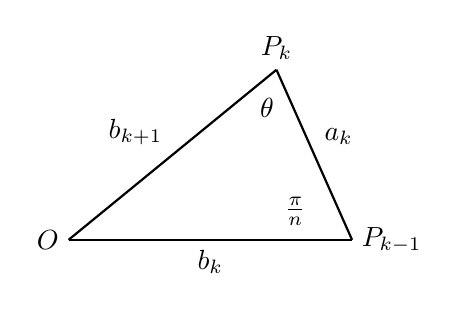
\begin{tikzpicture}[scale=1.2]
  \coordinate (O) at (0,0);
  \coordinate (Pk1) at (3,0);
  \coordinate (Pk) at (2.2, 1.8);
  \draw[thick] (O) -- (Pk1) node[midway, below] {$b_k$};
  \draw[thick] (O) -- (Pk) node[midway, above left] {$b_{k+1}$};
  \draw[thick] (Pk1) -- (Pk) node[midway, above right] {$a_k$};
  \node[left] at (O) {$O$};
  \node[right] at (Pk1) {$P_{k-1}$};
  \node[above] at (Pk) {$P_k$};
  \node at (2.4, 0.3) {$\frac{\pi}{n}$};
  \node at (2.1, 1.4) {$\theta$};
\end{tikzpicture}
\end{center}

\[
\frac{a_k}{\sin \frac{\pi}{n}} = \frac{b_{k+1}}{\sin \theta} = \frac{b_k}{\sin\left(\theta + \frac{\pi}{n}\right)} \quad \cdots ①
\]
①から
\[
b_{k+1} = \frac{\sin \theta}{\sin\left(\theta + \frac{\pi}{n}\right)} b_k \quad \cdots \text{\textcircled{イ}}
\]
又 ②から $b_1 = 1, b_2 = 1 + \frac{1}{n}$ だから, \textcircled{イ} で $k=1$ として

\begin{center}
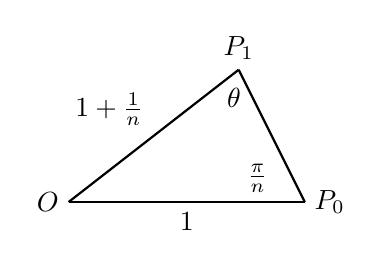
\begin{tikzpicture}[scale=1.2]
  \coordinate (O) at (0,0);
  \coordinate (P0) at (2.5,0);
  \coordinate (P1) at (1.8,1.4);
  \draw[thick] (O) -- (P0) node[midway, below] {$1$};
  \draw[thick] (O) -- (P1) node[midway, above left] {$1+\frac{1}{n}$};
  \draw[thick] (P0) -- (P1);
  \node[left] at (O) {$O$};
  \node[right] at (P0) {$P_0$};
  \node[above] at (P1) {$P_1$};
  \node at (2.0, 0.25) {$\frac{\pi}{n}$};
  \node at (1.75, 1.1) {$\theta$};
\end{tikzpicture}
\end{center}

\[
1 + \frac{1}{n} = \frac{\sin \theta}{\sin\left(\theta + \frac{\pi}{n}\right)} \quad \cdots \text{\textcircled{ウ}}
\]
\textcircled{イ}, \textcircled{ウ} と上記の初期条件から
\[
b_k = \left(1 + \frac{1}{n}\right)^{k-1} \quad \cdots \text{\textcircled{エ}}
\]
$\alpha = 1 + \frac{1}{n}$ として $\triangle O P_k P_{k-1}$ に余弦定理を用いて
\[
a_k = \alpha^{k-1} \sqrt{1 + \alpha^2 - 2\alpha \cos \frac{\pi}{n}}
\]
だから
\[
S_n = \frac{1 - \alpha^n}{1 - \alpha} \sqrt{1 + \alpha^2 - 2\alpha \cos \frac{\pi}{n}}
\]
$t = \frac{1}{n}$ とおいて整理する
\[
S_n = (\alpha^n - 1) \sqrt{ 2 \frac{1 - \cos t\pi}{t^2} + 1 + \frac{2(1 - \cos t\pi)}{t} }
\]
\[
\longrightarrow (e - 1) \sqrt{\pi^2 + 1} \quad (n \to \infty) \quad \text{//}
\]
\end{proof}

\end{document}
